% density_story.tex — risk-neutral density narrative for the LocalVolatility / Dupire-NN paper
% Authors: Wang Z., Shaa A., Privault N., Guet C.
% Build: cd presentation && pdflatex density_story.tex && pdflatex density_story.tex
\documentclass[aspectratio=169,11pt]{beamer}

\usetheme{default}
\setbeamertemplate{navigation symbols}{}
\setbeamertemplate{footline}{}

\usepackage{booktabs}
\usepackage{amsmath,amssymb,amsfonts}
\usepackage{mathtools}
\usepackage{bm}
\usepackage{tikz}
\usetikzlibrary{shapes,arrows,positioning,calc}
\usepackage{xcolor}
\usepackage{graphicx}
\usepackage{hyperref}

\graphicspath{{figures/}{figures/dec10_pdfs/}}

\definecolor{ntunavy}{RGB}{0,32,91}
\definecolor{ntudarkblue}{RGB}{0,20,60}
\definecolor{ntured}{RGB}{192,32,38}
\definecolor{ntugold}{RGB}{255,204,0}
\definecolor{ntulightblue}{RGB}{100,150,200}

\setbeamercolor{background canvas}{bg=ntunavy}
\setbeamercolor{normal text}{fg=white}
\setbeamercolor{frametitle}{fg=white}
\setbeamercolor{title}{fg=white}
\setbeamercolor{subtitle}{fg=ntugold}
\setbeamercolor{author}{fg=ntugold}
\setbeamercolor{institute}{fg=white}
\setbeamercolor{date}{fg=ntured}
\setbeamercolor{item}{fg=ntugold}
\setbeamercolor{structure}{fg=ntugold}
\setbeamercolor{block title}{fg=white,bg=ntured}
\setbeamercolor{block body}{fg=white,bg=ntunavy!70!black}

\setbeamerfont{title}{size=\Large,series=\bfseries}
\setbeamerfont{frametitle}{size=\large,series=\bfseries}
\setbeamertemplate{itemize item}{\scriptsize\raise1.5pt\hbox{\textbullet}}

\newcommand{\vect}[1]{\bm{#1}}

\setbeamertemplate{background}{
    \begin{tikzpicture}[remember picture,overlay]
        \shade[left color=ntunavy,right color=ntudarkblue,shading angle=-45]
            (current page.north west) rectangle (current page.south east);
        \fill[ntured]
            (current page.north west) --
            ([xshift=1.8cm]current page.north west) --
            ([yshift=-2.7cm]current page.north west) -- cycle;
        \fill[ntured!85!black]
            ([yshift=-2.2cm]current page.north west) --
            ([xshift=1.4cm,yshift=-2.2cm]current page.north west) --
            ([yshift=-4.0cm]current page.north west) -- cycle;
    \end{tikzpicture}
}

\defbeamertemplate*{title page}{ntu}[1][]
{
    \begin{tikzpicture}[remember picture,overlay]
        \shade[left color=ntunavy,right color=ntudarkblue!90!ntunavy,shading angle=-30]
            (current page.north west) rectangle (current page.south east);
        \fill[ntured]
            (current page.north west) --
            ([xshift=2.2cm]current page.north west) --
            ([yshift=-3.3cm]current page.north west) -- cycle;
        \IfFileExists{ntu_logo.jpg}{
            \node[anchor=north west] at ([xshift=0.5cm,yshift=-0.4cm]current page.north west) {
                
\includegraphics[height=1.2cm]{ntu_logo.jpg}
            };
        }{}
        \node[anchor=north west, text width=10cm, font=\fontsize{11}{13}\selectfont\bfseries]
            at ([xshift=2.8cm,yshift=-2.3cm]current page.north west) {
            \textcolor{ntugold}{Dupire PINN / PDF validation}
        };
        \node[anchor=north west, text width=10.5cm]
            at ([xshift=2.8cm,yshift=-3.0cm]current page.north west) {
            {\fontsize{20}{24}\selectfont\bfseries\color{white}\inserttitle}
        };
        \node[anchor=north west, text width=10cm, font=\fontsize{12}{14}\selectfont\bfseries]
            at ([xshift=2.8cm,yshift=-5.4cm]current page.north west) {
            \textcolor{ntugold}{\insertauthor}
        };
        \node[anchor=north west, text width=10cm, font=\fontsize{8}{10}\selectfont]
            at ([xshift=2.8cm,yshift=-6.0cm]current page.north west) {
            \textcolor{white}{\insertinstitute}
        };
        \node[anchor=north west, font=\fontsize{10}{12}\selectfont\bfseries]
            at ([xshift=2.8cm,yshift=-7.2cm]current page.north west) {
            \textcolor{ntured}{\insertdate}
        };
    \end{tikzpicture}
}

\setbeamertemplate{frametitle}{
    \vspace{0.3cm}
    \hspace{2.5cm}{\usebeamerfont{frametitle}\insertframetitle}
    \vspace{0.1cm}
}

\title{The risk-neutral density and the $K\!=\!0$ boundary:\\derivation, observation, diagnosis}
\subtitle{Wang Z., Shaa A., Privault N., Guet C.}
\author{Ameir Shaa}
\date{\today}
\institute{JCF manuscript --- LocalVolatility PINN pipeline}

% ============================================================
\begin{document}
\maketitle

\begin{frame}{Outline}
  \tableofcontents
\end{frame}

% ============================================================
\section{The risk-neutral density}

\begin{frame}{Setup: from option prices to a density}
  \[
    C(K,T) = e^{-rT}\,\mathbb{E}^{\mathbb{Q}}[(S_T-K)^+]
            = e^{-rT}\int_K^\infty (S-K)\,f(S)\,dS
  \]
  \begin{itemize}
    \item $f$ is the (unknown) risk-neutral density of $S_T$. Goal: recover $f$ from
          prices, then check it against Monte-Carlo simulation of the calibrated model.
    \item Our NN parameterizes $C$; the implied density follows by differentiation
          (next slide).
  \end{itemize}
\end{frame}

\begin{frame}{Breeden--Litzenberger: the density is $\partial^2 C/\partial K^2$}
  Differentiate under the integral (Leibniz; the lower-limit boundary term vanishes
  since the integrand $(S-K)$ is zero at $S=K$):
  \begin{align*}
    \frac{\partial C}{\partial K}
      &= -e^{-rT}\int_K^\infty f(S)\,dS
       = -e^{-rT}\bigl(1-F(K)\bigr)
       = -e^{-rT}\,\mathbb{Q}(S_T>K),\\[4pt]
    \frac{\partial^2 C}{\partial K^2}
      &= e^{-rT}\,f(K).
  \end{align*}
  \[
    \boxed{\,q(K,T) \;:=\; e^{rT}\,\frac{\partial^2 C}{\partial K^2}(K,T) \;=\; f_{\mathbb{Q}}(K)\,}
  \]
  {\footnotesize Regularity: $f$ integrable, $C\to 0$ and $\partial_K C\to 0$ as $K\to\infty$.}
\end{frame}

\begin{frame}{The mean identity (integration by parts)}
  \[
    \mathbb{E}[S_T]
      = \int_0^\infty K\,q(K,T)\,dK
      = e^{rT}\int_0^\infty K\,\frac{\partial^2 C}{\partial K^2}\,dK
  \]
  IBP:
  \[
    \int_0^\infty K\,\frac{\partial^2 C}{\partial K^2}\,dK
      = \Bigl[K\,\frac{\partial C}{\partial K}-C\Bigr]_0^\infty
      = C(0,T) = S_0
  \]
  (at $\infty$: $C\to 0$, $K\partial_K C\to 0$; at $0$: $K\partial_K C\to 0$ and
  $C(0,T)=S_0$, the zero-strike call equals spot).
  \[
    \boxed{\,\mathbb{E}[S_T] = e^{rT}C(0,T) = S_0\,e^{rT}\,}
  \]
  Three independent estimators that must all equal the forward
  $M_{\mathrm{ref}}=S_0 e^{rT}$:
  \begin{itemize}
    \item $M_1 = e^{rT}\!\int_0^\infty K\,\partial^2_K C\,dK$ \quad(density quadrature),
    \item $M_2 = e^{rT}C(0,T)$ \quad(closed form),
    \item $M_3 = \mathbb{E}[S_T]$ \quad(Monte Carlo).
  \end{itemize}
\end{frame}

% ============================================================
\section{December observations: a deviation}

\begin{frame}{What we plot}
  For each maturity $T$, three panels:
  \begin{enumerate}
    \item Strike-space density $f(K)$ --- MC histogram vs NN model vs analytical.
    \item Log-strike density $f(\ln K)$.
    \item Gaussian space --- standardized MC (KDE) vs NN, against $\mathcal{N}(0,1)$.
  \end{enumerate}
  \vspace{0.4em}
  The NN curve is the Breeden--Litzenberger density
  $e^{rT}\partial^2_K C_{\mathrm{NN}}$; the MC histogram is the simulated $S_T$
  under the calibrated $\sigma_{\mathrm{NN}}$.
\end{frame}

\begin{frame}{Control: constant volatility $\sigma=1$}
  \begin{center}
    \includegraphics[width=0.93\linewidth,height=0.74\textheight,keepaspectratio]{syn_const_sigma.png}
  \end{center}
  {\footnotesize $T\in\{0.25,0.5,0.75,1.0\}$. NN, MC and the log-normal analytical density are
  essentially indistinguishable --- the clean baseline, no deviation.}
\end{frame}

\begin{frame}{Synthetic Dupire volatility}
  \begin{center}
    \includegraphics[width=0.93\linewidth,height=0.74\textheight,keepaspectratio]{syn_dupire_nonconst.png}
  \end{center}
  {\footnotesize $\sigma(x,t)=0.3+y e^{-y}$,\,$y=(t{+}0.1)\sqrt{x{+}0.1}$. NN tracks MC
  closely; a small deficit is already visible in the Gaussian panel.}
\end{frame}

\begin{frame}{Market data: DAX 7 Aug 2001}
  \begin{center}
    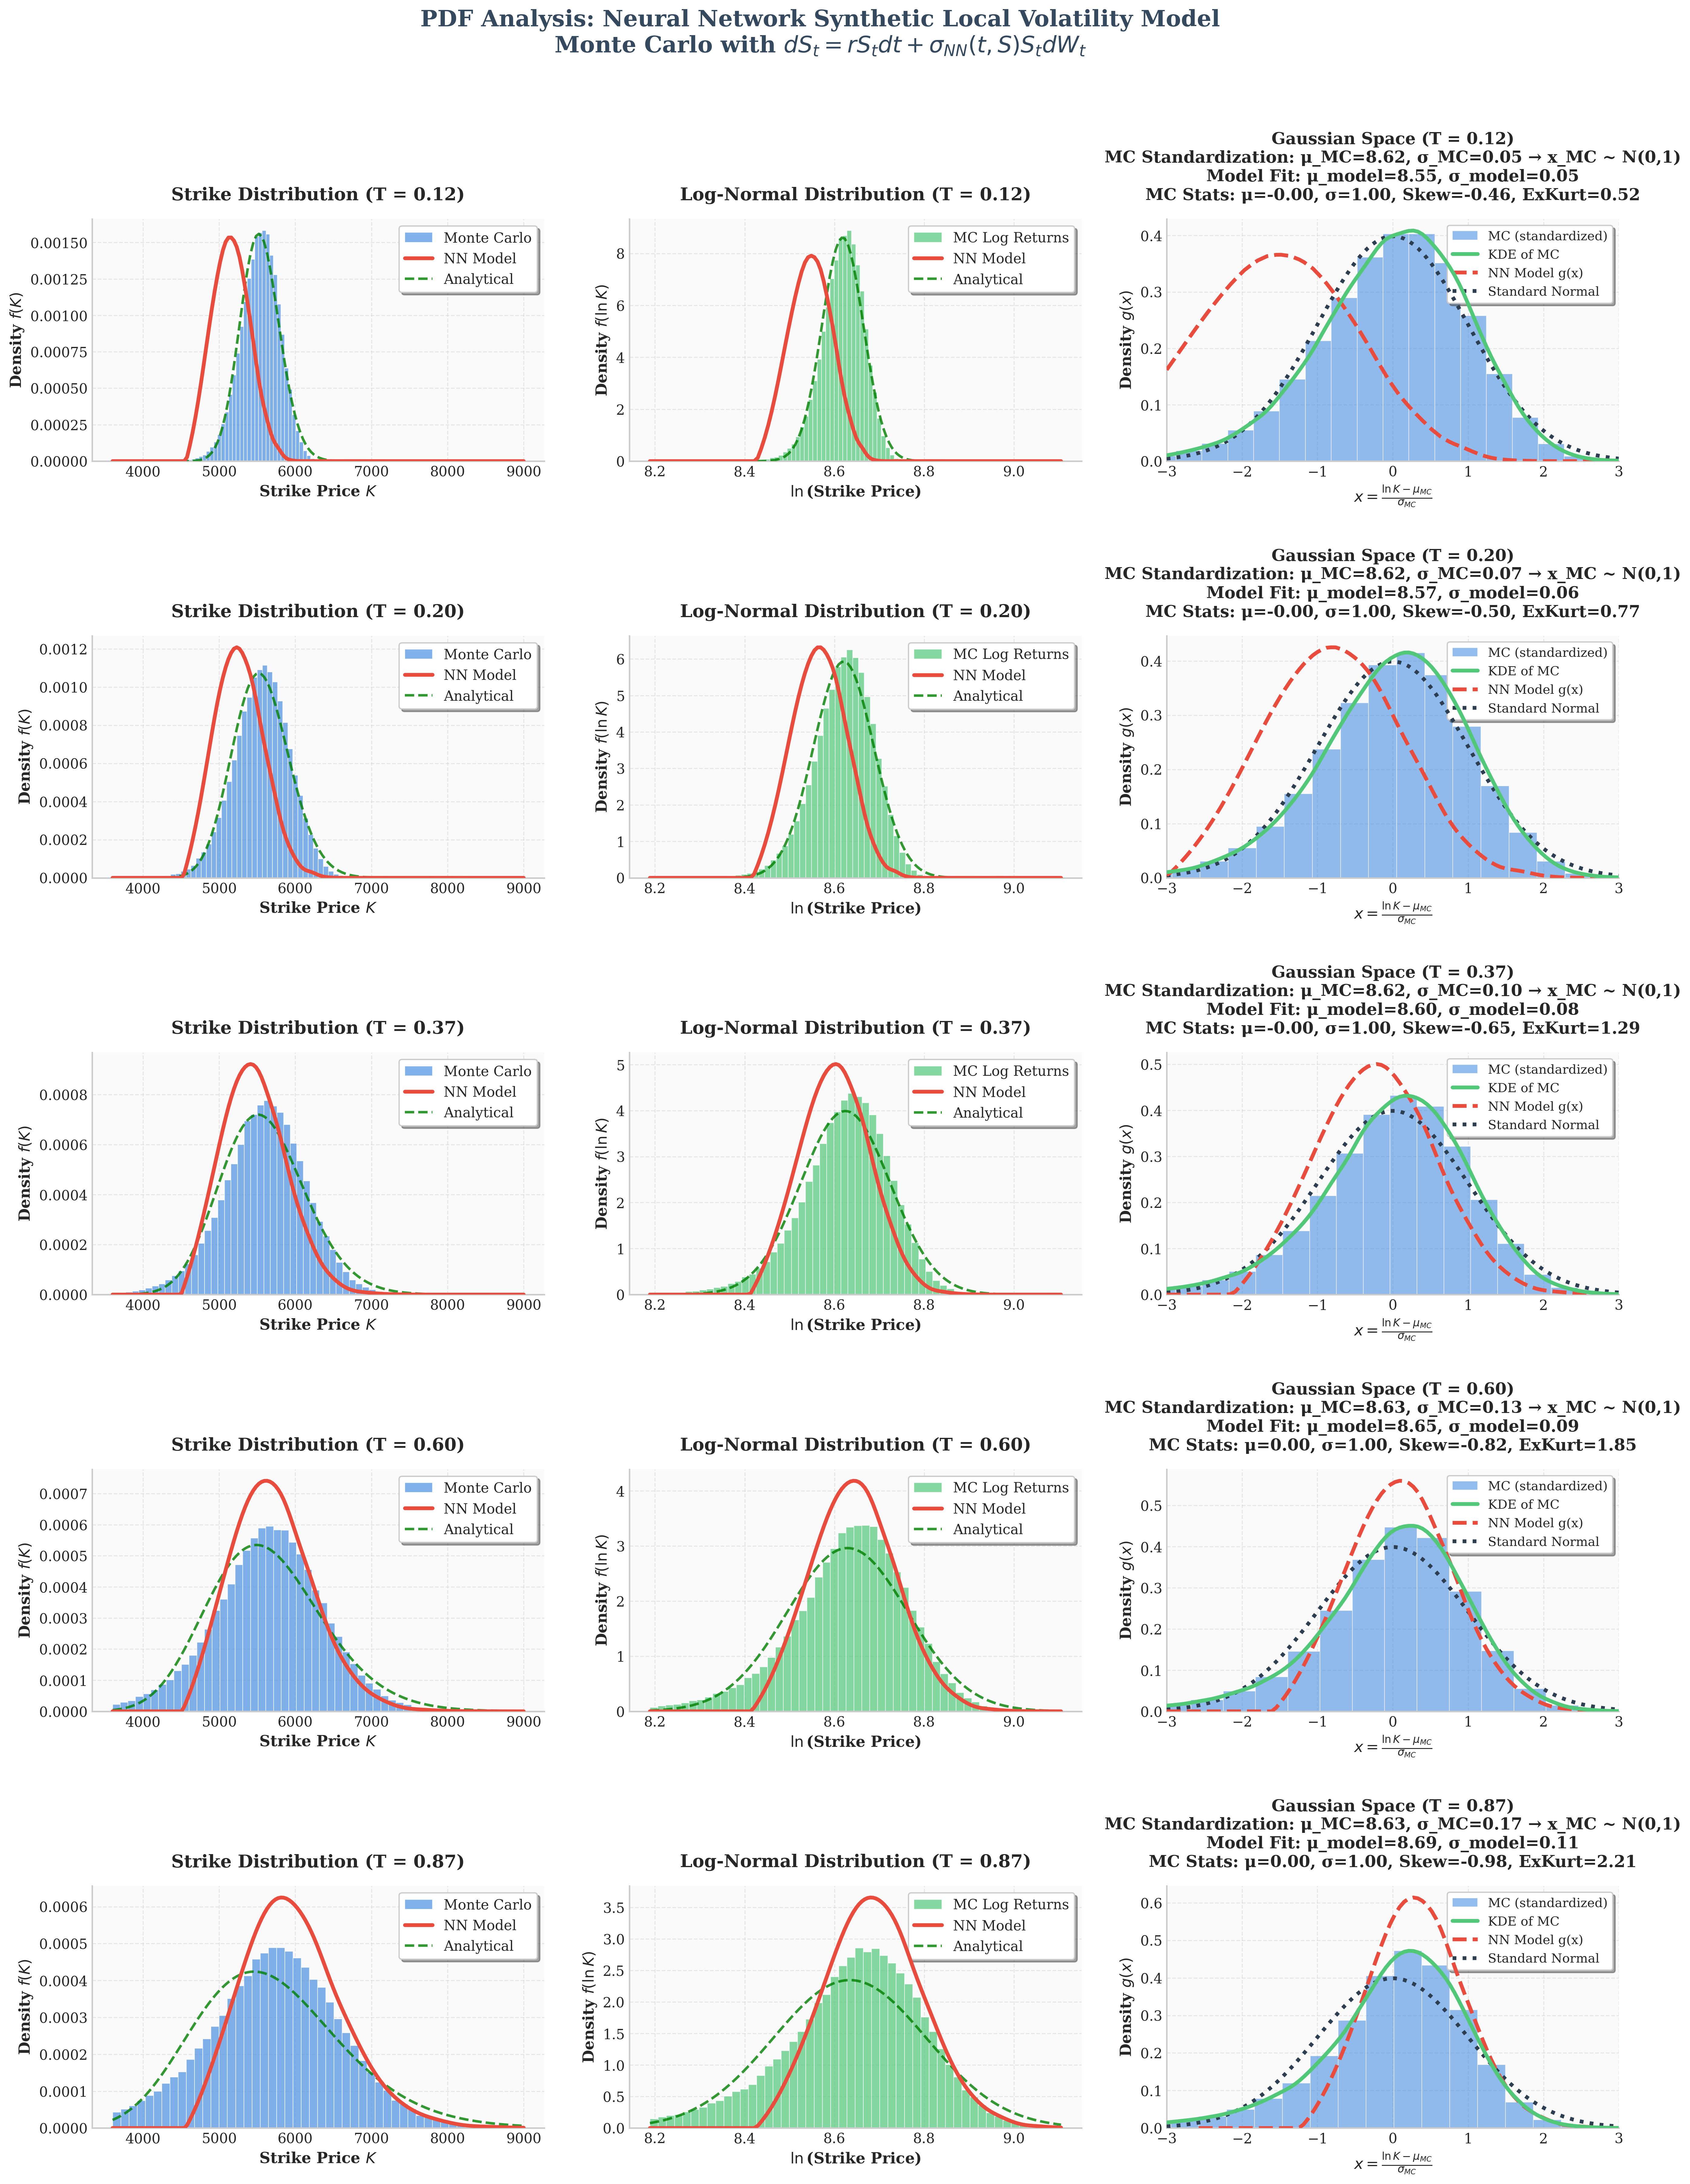
\includegraphics[width=0.93\linewidth,height=0.74\textheight,keepaspectratio]{dax_day1_aug7.png}
  \end{center}
  {\footnotesize $K\in[4000,9000]$, $T\in\{0.12,0.20,0.37,0.60,0.87\}$. Clear NN-vs-MC
  separation in strike space; in Gaussian space MC tracks $\mathcal{N}(0,1)$ but the
  NN density deviates --- the $K{=}0$ boundary fingerprint.}
\end{frame}

\begin{frame}{DAX 8--9 Aug 2001: consistent across days}
  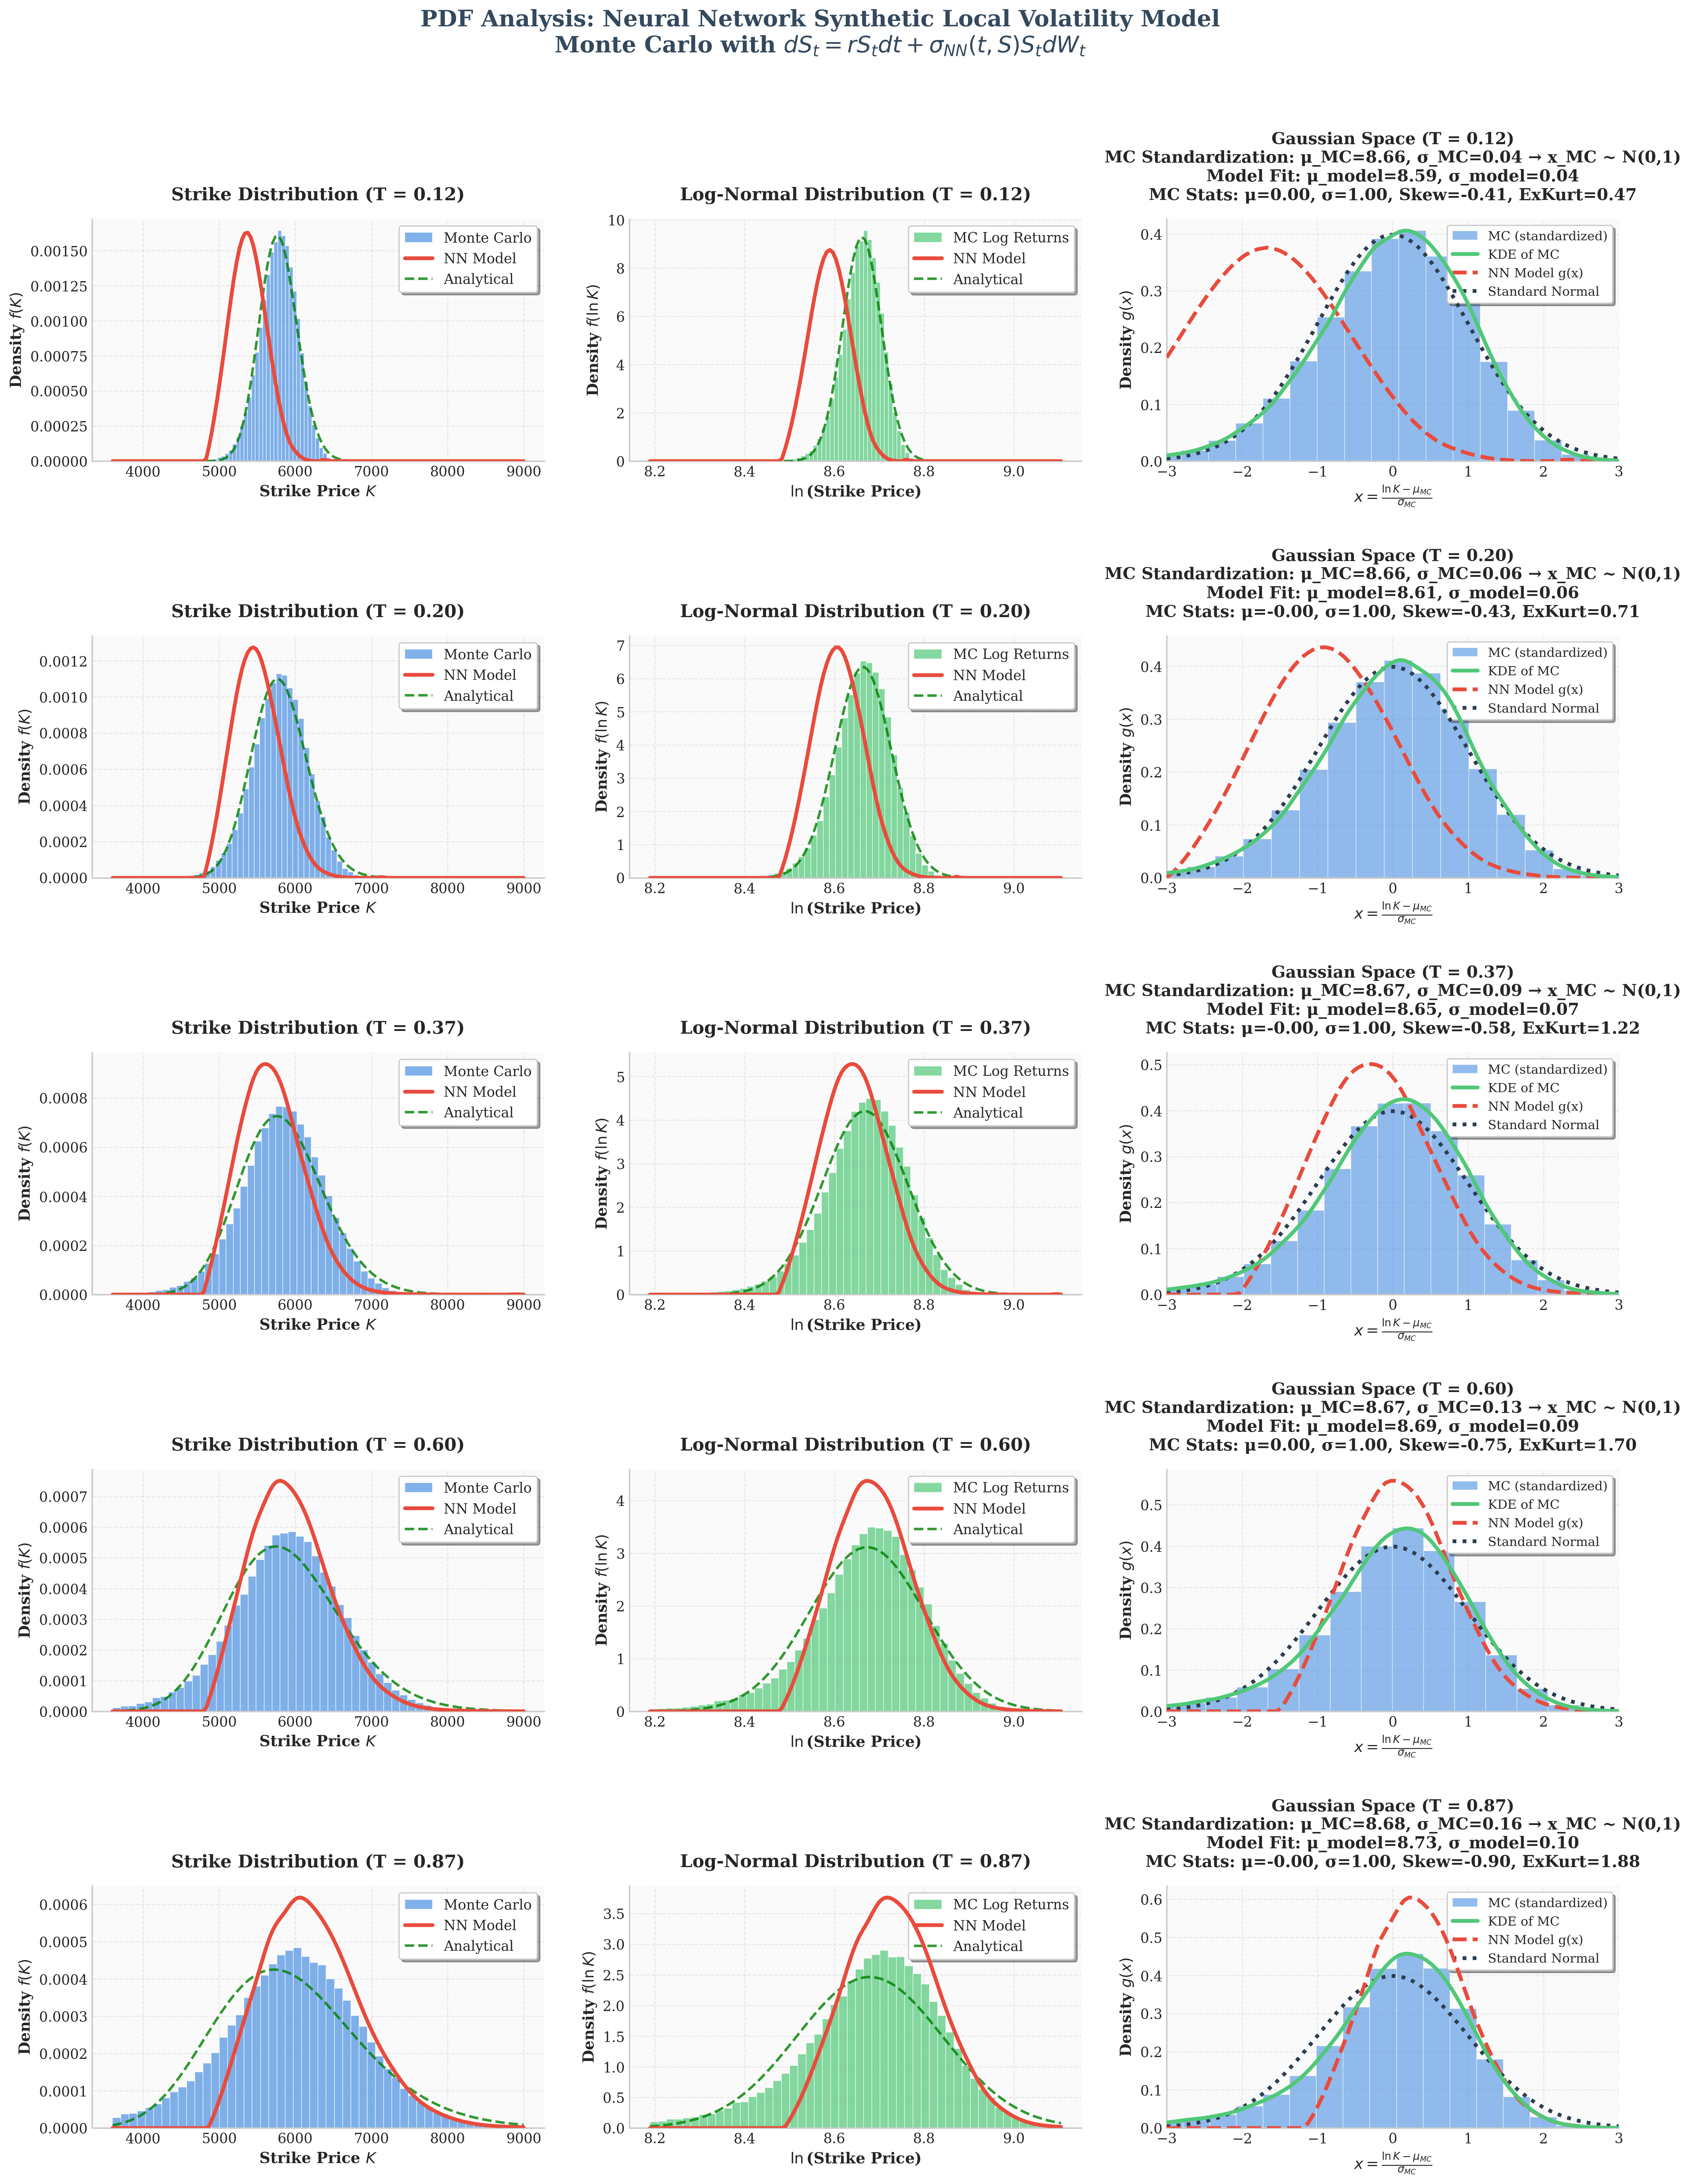
\includegraphics[width=0.48\linewidth]{dax_day2_aug8.png}\hfill
  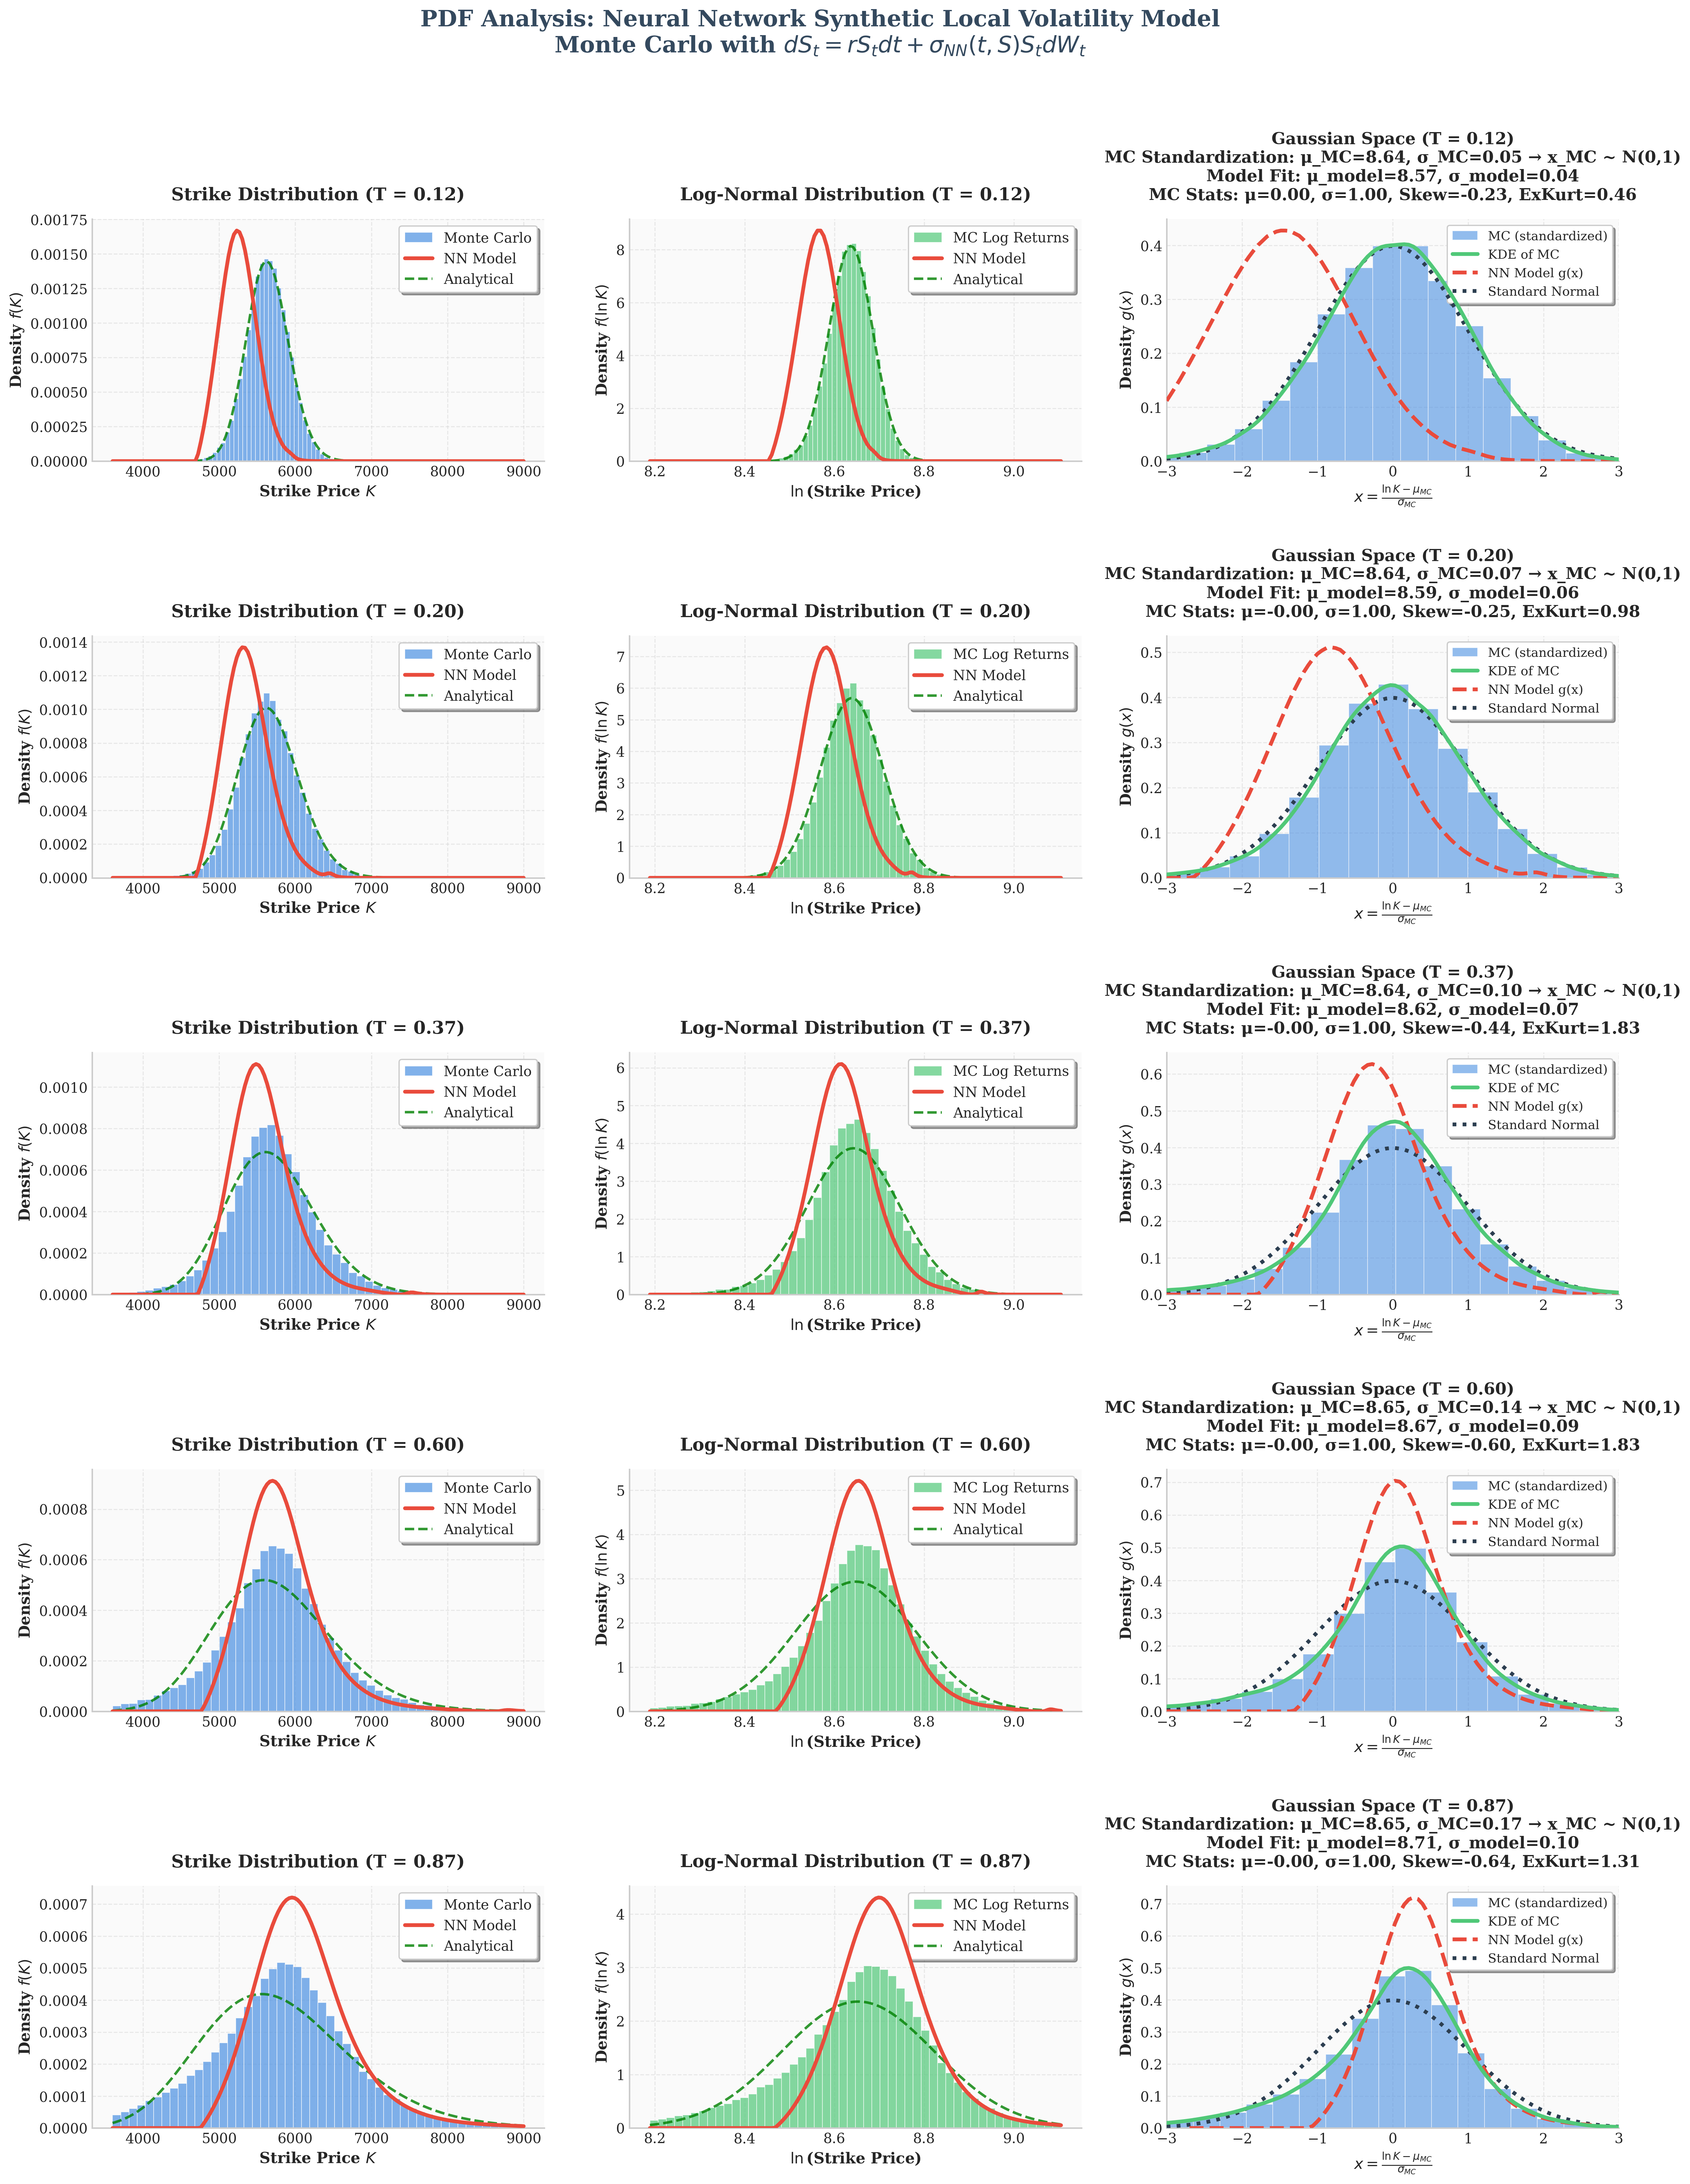
\includegraphics[width=0.48\linewidth]{dax_day3_aug9.png}

  \vspace{0.3em}
  {\footnotesize Same structural NN-vs-MC deviation on Aug 8 (left) and Aug 9 (right)
  --- the effect is systematic, not a one-day artefact. \emph{Provisional day
  assignment.}}

  \vspace{0.3em}
  The deviation is real and structural. Where does it come from?
\end{frame}

% ============================================================
\section{The NN density in scaled coordinates}

\begin{frame}{The scaling the network uses}
  \[
    t=\frac{T}{T_{\max}},\qquad
    k=\frac{e^{-rT}K}{K_{\max}},\qquad
    \tilde\varphi=\frac{C}{S_0},\qquad
    \eta=\tfrac{1}{2}\,T_{\max}\,\sigma^2
  \]
  Price ansatz (as trained):
  \[
    \tilde\varphi(k,t) = 1 - e^{-\mathcal{N}_c(k,t)},\qquad
    \mathcal{N}_c = \mathrm{NN}_\varphi\ \text{(softplus output, }>0).
  \]
\end{frame}

\begin{frame}{Rederiving the density under the scaling}
  The map $K\mapsto k$ is linear, so the Jacobian is constant:
  \[
    \frac{dk}{dK}=\frac{e^{-rT}}{K_{\max}},\qquad
    \frac{d^2k}{dK^2}=0.
  \]
  Hence (no curvature term):
  \[
    \frac{\partial^2 C}{\partial K^2}
      = S_0\Bigl(\frac{dk}{dK}\Bigr)^2\frac{\partial^2\tilde\varphi}{\partial k^2}.
  \]
  \[
    \boxed{\,q(K,T)=e^{rT}\frac{\partial^2 C}{\partial K^2}
      =e^{rT}S_0\Bigl(\frac{e^{-rT}}{K_{\max}}\Bigr)^2\frac{\partial^2\tilde\varphi}{\partial k^2}
      =\frac{S_0\,e^{-rT}}{K_{\max}^2}\frac{\partial^2\tilde\varphi}{\partial k^2}\,}
  \]
  {\footnotesize Scaled Dupire PDE: $\partial_t\varphi=\eta(k,t)\,k^2\,\partial_k^2\varphi$.}
\end{frame}

\begin{frame}{Implementation verified}
  \begin{itemize}
    \item This boxed formula is exactly what \texttt{\_raw\_model\_density} computes
          (double autodiff for $\partial_k^2\tilde\varphi$, Jacobian
          $(e^{-rT}/K_{\max})^2$, $\times S_0$, $\times e^{rT}$).
    \item The density and IBP-diagnostic code
          (\texttt{\_raw\_model\_density},
          \texttt{compute\_mean\_diagnostics},
          \texttt{prepare\_data\_for\_nn},
          \texttt{phi\_tilde\_from\_nn})
          were audited line-by-line against the math above --- Jacobian power, a
          single $e^{rT}$, the $S_0$ factor --- and all match.
    \item Numerically re-checked: the autodiff second derivative and the trapezoidal
          quadrature are mutually consistent --- $M_1\equiv M_2$ to machine precision
          (the IBP identity; see next section).
  \end{itemize}
  \vspace{0.3em}
  {\footnotesize The code is correct; the residual the diagnostic exposes is a property
  of the trained \emph{model}, not of its implementation.}
\end{frame}

% ============================================================
\section{IBP sanity checks}

\begin{frame}{Three-way check (pretrained, synthetic Dupire surface)}
  \footnotesize
  \setlength{\tabcolsep}{4pt}
  \centering
  \begin{tabular}{r r r r r r r r r r}
    \toprule
    $T$ & $M_{\mathrm{ref}}$ & $M_1$ & \%err & $M_2$ & \%err & $M_3$ & \%err
        & $\Delta M_{12}\%$ & $\Delta M_{13}\%$ \\
    \midrule
    0.5 & 1020.20 & 948.87 & $-6.99$ & 948.93 & $-6.99$ & 1018.25 & $-0.19$
        & 0.006 & 6.814 \\
    1.0 & 1040.81 & 967.66 & $-7.03$ & 967.74 & $-7.02$ & 1038.19 & $-0.25$
        & 0.009 & 6.794 \\
    1.5 & 1061.84 & 982.49 & $-7.47$ & 982.95 & $-7.43$ & 1054.36 & $-0.70$
        & 0.047 & 6.816 \\
    \bottomrule
  \end{tabular}
  \vspace{0.4em}
  \scriptsize
  \begin{itemize}
    \item $M_1\equiv M_2$ to $<0.05\%$: autodiff + quadrature consistent (IBP identity exact).
    \item $M_3$ within $0.7\%$ of forward: $\mathrm{NN}_\eta$ (the vol net) is
          well-calibrated.
    \item $M_1,M_2\approx 7\%$ below forward: $\mathrm{NN}_\varphi$ (the price net)
          undershoots near $K=0$.
  \end{itemize}
\end{frame}

\begin{frame}{$\Delta M_{12}$, $\Delta M_{13}$ vs maturity}
  \begin{center}
    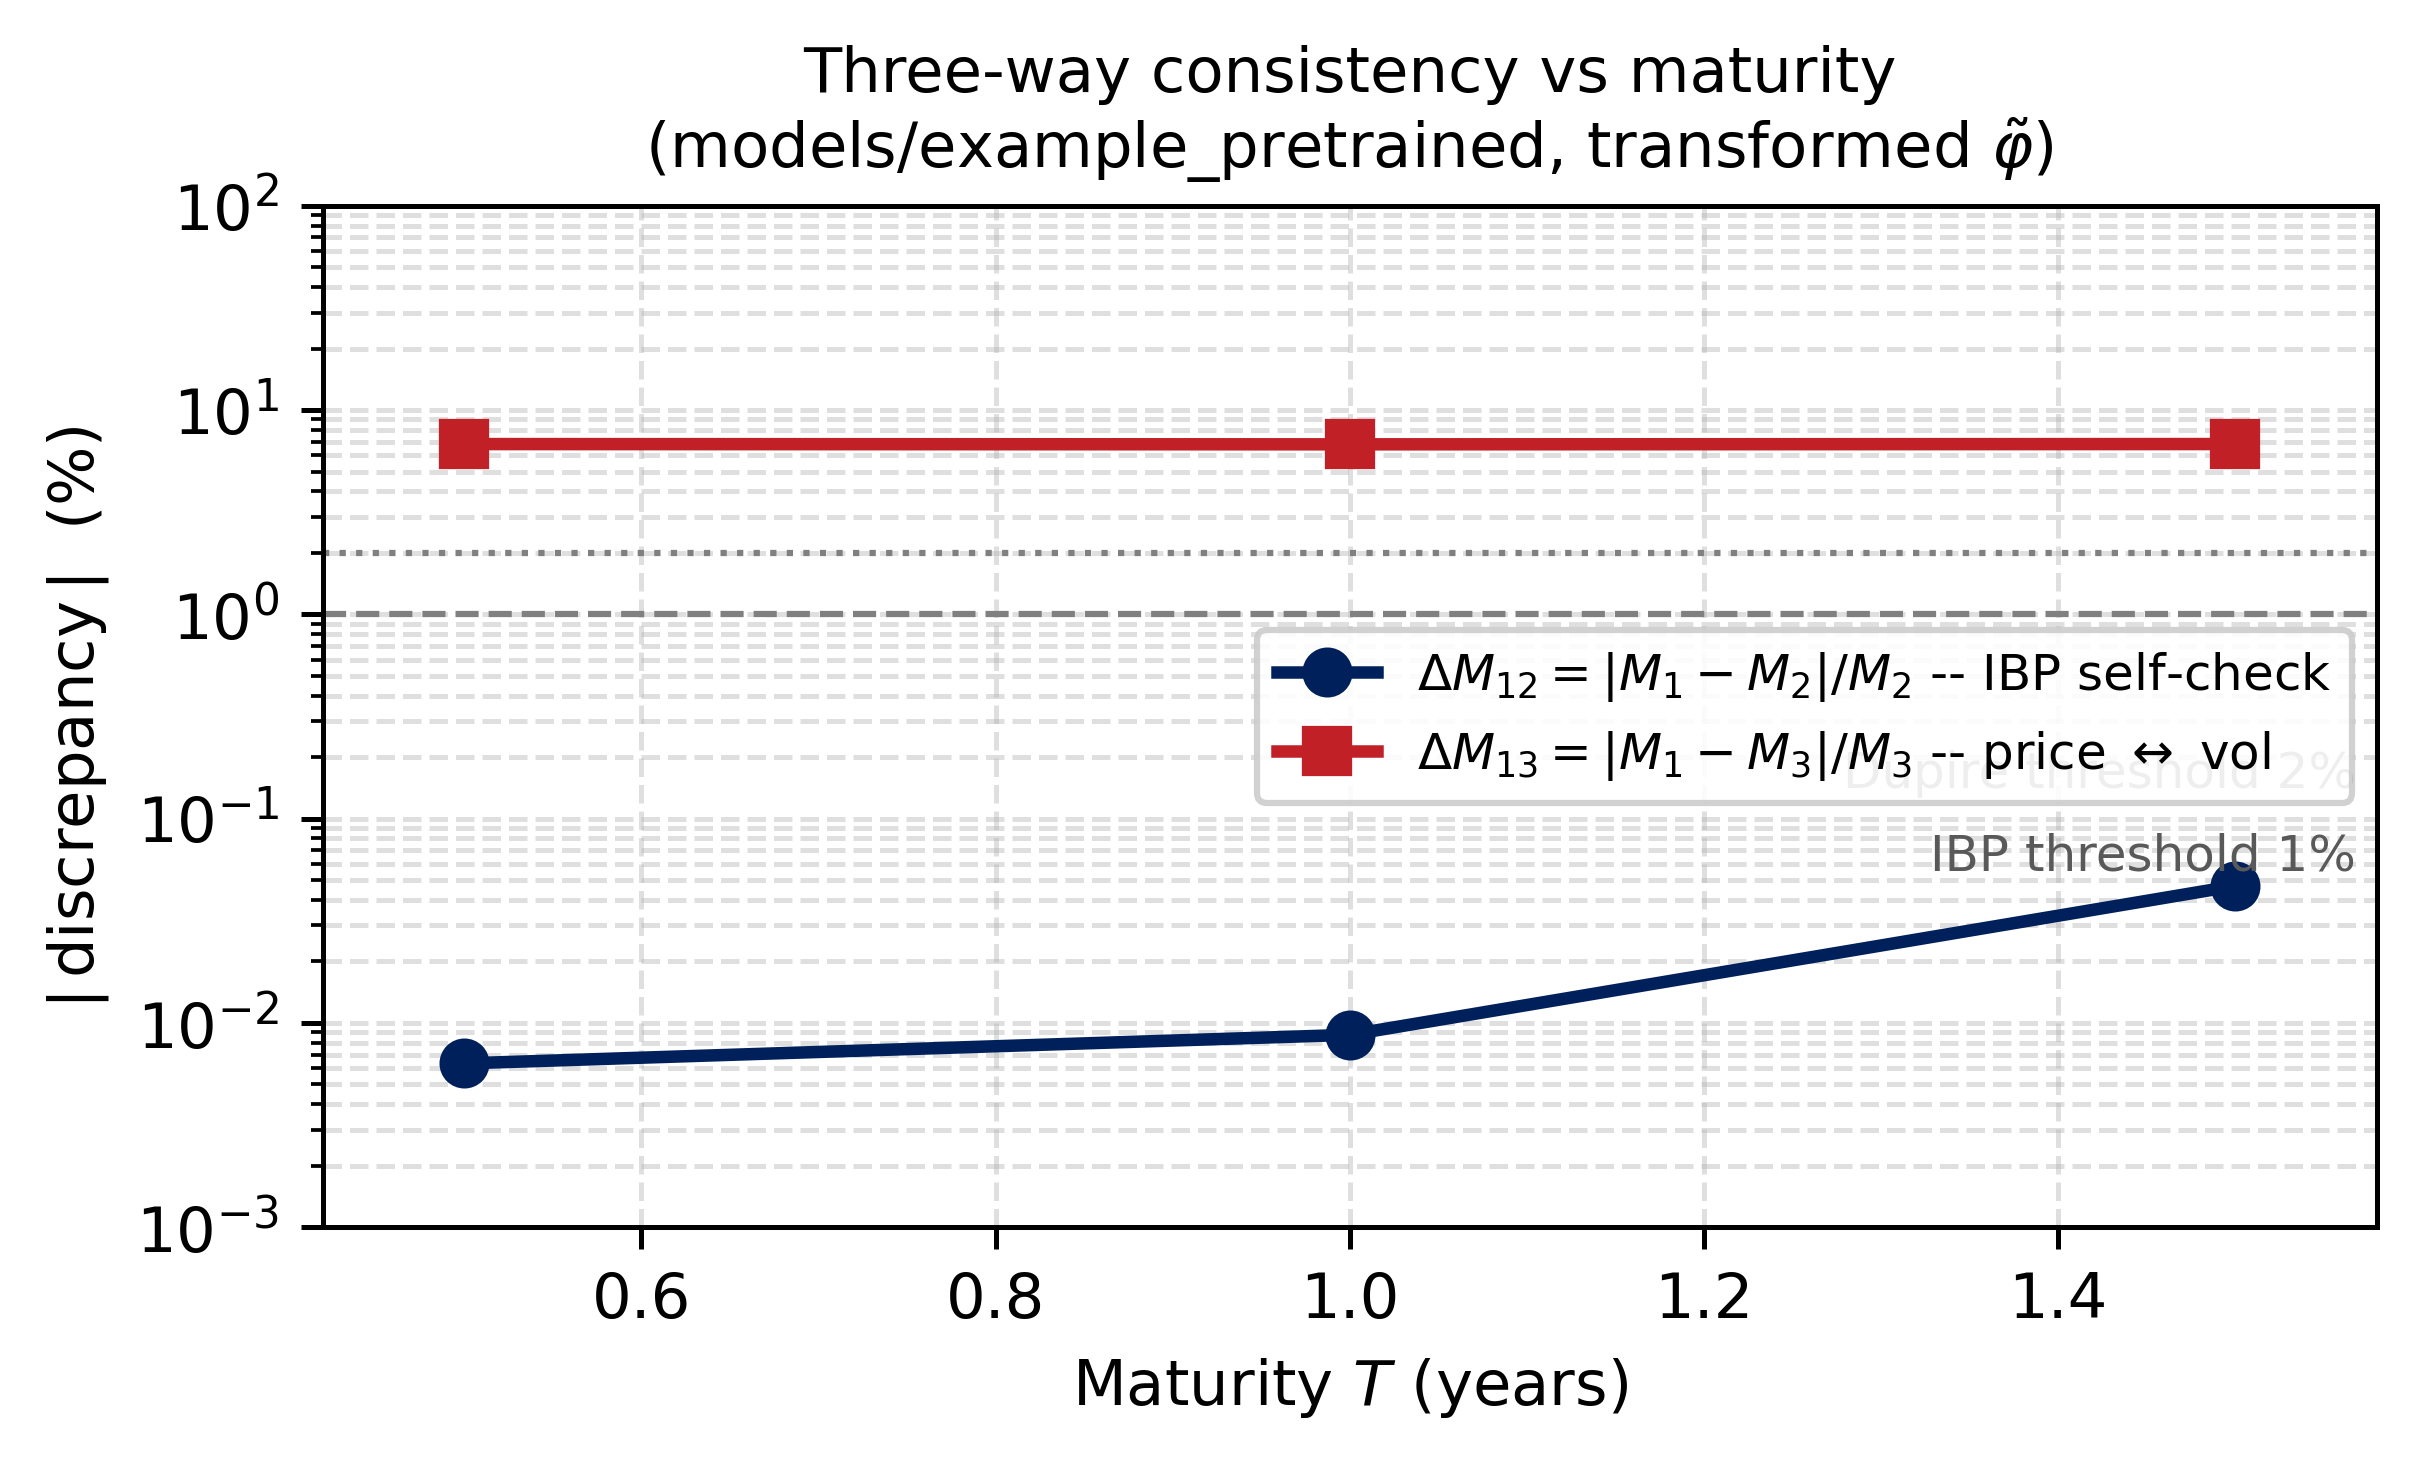
\includegraphics[width=0.78\linewidth,keepaspectratio]{ibp_deltas_vs_T.png}
  \end{center}
  {\footnotesize $\Delta M_{12}$ at machine precision (IBP exact); $\Delta M_{13}\approx7\%$,
  flat in $T$ --- a systematic price-net gap, not a calibration drift.}
\end{frame}

\begin{frame}{Direct check: NN output at the boundaries}
  \small
  Evaluating the trained network at $k=0$ and $k=1$:
  \vspace{0.3em}
  \setlength{\tabcolsep}{6pt}
  \centering
  \begin{tabular}{r r r r r r}
    \toprule
    $T$ & $\mathcal{N}_c(0,T)$ & $\tilde\varphi(0,T)$ & deficit
        & $\mathcal{N}_c(1,T)$ & $\tilde\varphi(1,T)$ \\
    \midrule
    0.5 & 2.661 & 0.9301 & $6.99\%$ & 0.0007 & 0.0007 \\
    1.0 & 2.656 & 0.9298 & $7.02\%$ & 0.0128 & 0.0128 \\
    1.5 & 2.600 & 0.9257 & $7.43\%$ & 0.0315 & 0.0310 \\
    \bottomrule
  \end{tabular}

  \vspace{0.3em}
  \begin{center}
    
\includegraphics[width=0.95\linewidth,height=0.40\textheight,keepaspectratio]{nn_at_k0.png}
  \end{center}
  {\footnotesize $\mathcal{N}_c(0,T)\approx2.6$ (finite --- would need $\infty$);
  $\mathcal{N}_c(1,T)\approx0.01$. $e^{rT}C_{\mathrm{NN}}(0,T)$ reproduces
  $M_2=948.9/967.7/983.0$.}
\end{frame}

\begin{frame}{Counterfactual: if the $(1-k)$ factor were present}
  \small
  Applying eq.~3.9's $(1-k)$ factor to the trained $\mathcal{N}_c$ at analysis time:
  \vspace{0.3em}
  \setlength{\tabcolsep}{6pt}
  \centering
  \begin{tabular}{r r r r r}
    \toprule
    $T$ & $M_2$ & $M_1^{\mathrm{cap}}$ & $M_1$ (pred) & $\Delta M_{12}^{\mathrm{cap}}\%$ \\
    \midrule
    0.5 & 948.93 & 948.25 & 948.22 & 0.072 \\
    1.0 & 967.74 & 954.37 & 954.42 & 1.381 \\
    1.5 & 982.95 & 949.51 & 949.50 & 3.402 \\
    \bottomrule
  \end{tabular}
  \vspace{0.3em}
  \scriptsize
  \begin{itemize}
    \item $k=0$: $M_2$ \textbf{unchanged} (factor $=1$ there) --- the $7\%$ deficit is identical.
    \item $k=1$: $\tilde\varphi$ forced to \textbf{exactly 0} by construction.
    \item But $M_1\neq M_2$: a real boundary-slope gap
          $=e^{rT}S_0\mathcal{N}_c(1)$, growing
          $0.07\%\to1.4\%\to3.4\%$ with $T$.
          Verified numerically (matches $M_2-e^{rT}S_0\mathcal{N}_c(1)$).
  \end{itemize}
\end{frame}

% ============================================================
\section{What went wrong}

\begin{frame}{The output map cannot reach $K\!=\!0$}
  \[
    \tilde\varphi = 1 - e^{-\mathcal{N}_c}\in(0,1),\qquad
    \mathcal{N}_c = \text{softplus}>0\ \Rightarrow\ \text{range open at }1.
  \]
  \begin{itemize}
    \item $K=\infty$ ($k=1$): BC $\tilde\varphi=0$ needs $\mathcal{N}_c=0$ ---
          \textbf{attainable} (measured $\approx0.01$).
    \item $K=0$ ($k=0$): BC $\tilde\varphi=1$ needs $\mathcal{N}_c\to\infty$ ---
          \textbf{unattainable} by a finite output (measured $\approx2.6$).
          So $C_{\mathrm{NN}}(0,T)<S_0$ by construction; the gap is the $7\%$.
  \end{itemize}
\end{frame}

\begin{frame}{Why the deficit is frozen in $T$}
  Scaled Dupire PDE:
  \[
    \frac{\partial\varphi}{\partial t} = \eta(k,t)\,k^2\,\frac{\partial^2\varphi}{\partial k^2}.
  \]
  At $k=0$ the $k^2$ factor annihilates the RHS, so
  $\partial_t\varphi(0,t)=0 \Rightarrow \varphi(0,t)=\varphi(0,0)\ \forall t$.

  \vspace{0.5em}
  The $T=0$ initial-condition deficit (which a finite ansatz cannot avoid) is
  propagated \textbf{unchanged} to every maturity --- exactly the flat
  $\Delta M_{13}\approx7\%$.
\end{frame}

\begin{frame}{Summary: the $(1-k)$ factor is not the fix}
  \begin{itemize}
    \item The deviation seen in December is the $\mathrm{NN}_\varphi$ $K{=}0$
          undershoot, localized by the IBP three-way test;
          $\mathrm{NN}_\eta$ is fine ($M_3$ on the forward).
    \item The manuscript's $(1-k)$ factor only pins $K=\infty$; at $k=0$ it is
          $1$, so the $7\%$ deficit is identical --- and it introduces a new
          $M_1\neq M_2$ gap.
    \item Fixes: a $K{=}0$ penalty
          $\lambda_{k_0}|C(0,T)-S_0|^2$ in the loss, or an ansatz that can
          attain $\tilde\varphi=1$, e.g. the parity form
          $\pi^c = S_0 - Ke^{rT}\bigl[1-(1-k)e^{-\mathcal{N}_c}\bigr]$
          (pins \emph{both} ends by construction).
  \end{itemize}
\end{frame}

% ============================================================
\begin{frame}{}
  \begin{center}
    \vspace{2cm}
    {\Huge\bfseries\color{white} Questions?}
    \vspace{0.5cm}
    {\large\color{ntugold}Plots: \texttt{plots/ibp\_comparison/}}
  \end{center}
\end{frame}

\end{document}
